\newcommand{\doctorDescription}{
\section{Healer}
\epigraph{\textit{
    "healer quote"
} }{
    healer quotee
}
    Some Description
    \\
    See \nref{tlttree:doctor} for more information.
}

\newcommand{\doctorTree}{
    \newpage
    \subsection{Healer Talent Tree}
    \label{tlttree:doctor}

    \textbf{Class Skills:} Cool, Medicine, Resilience, Knowledge (Education)
    \newline

    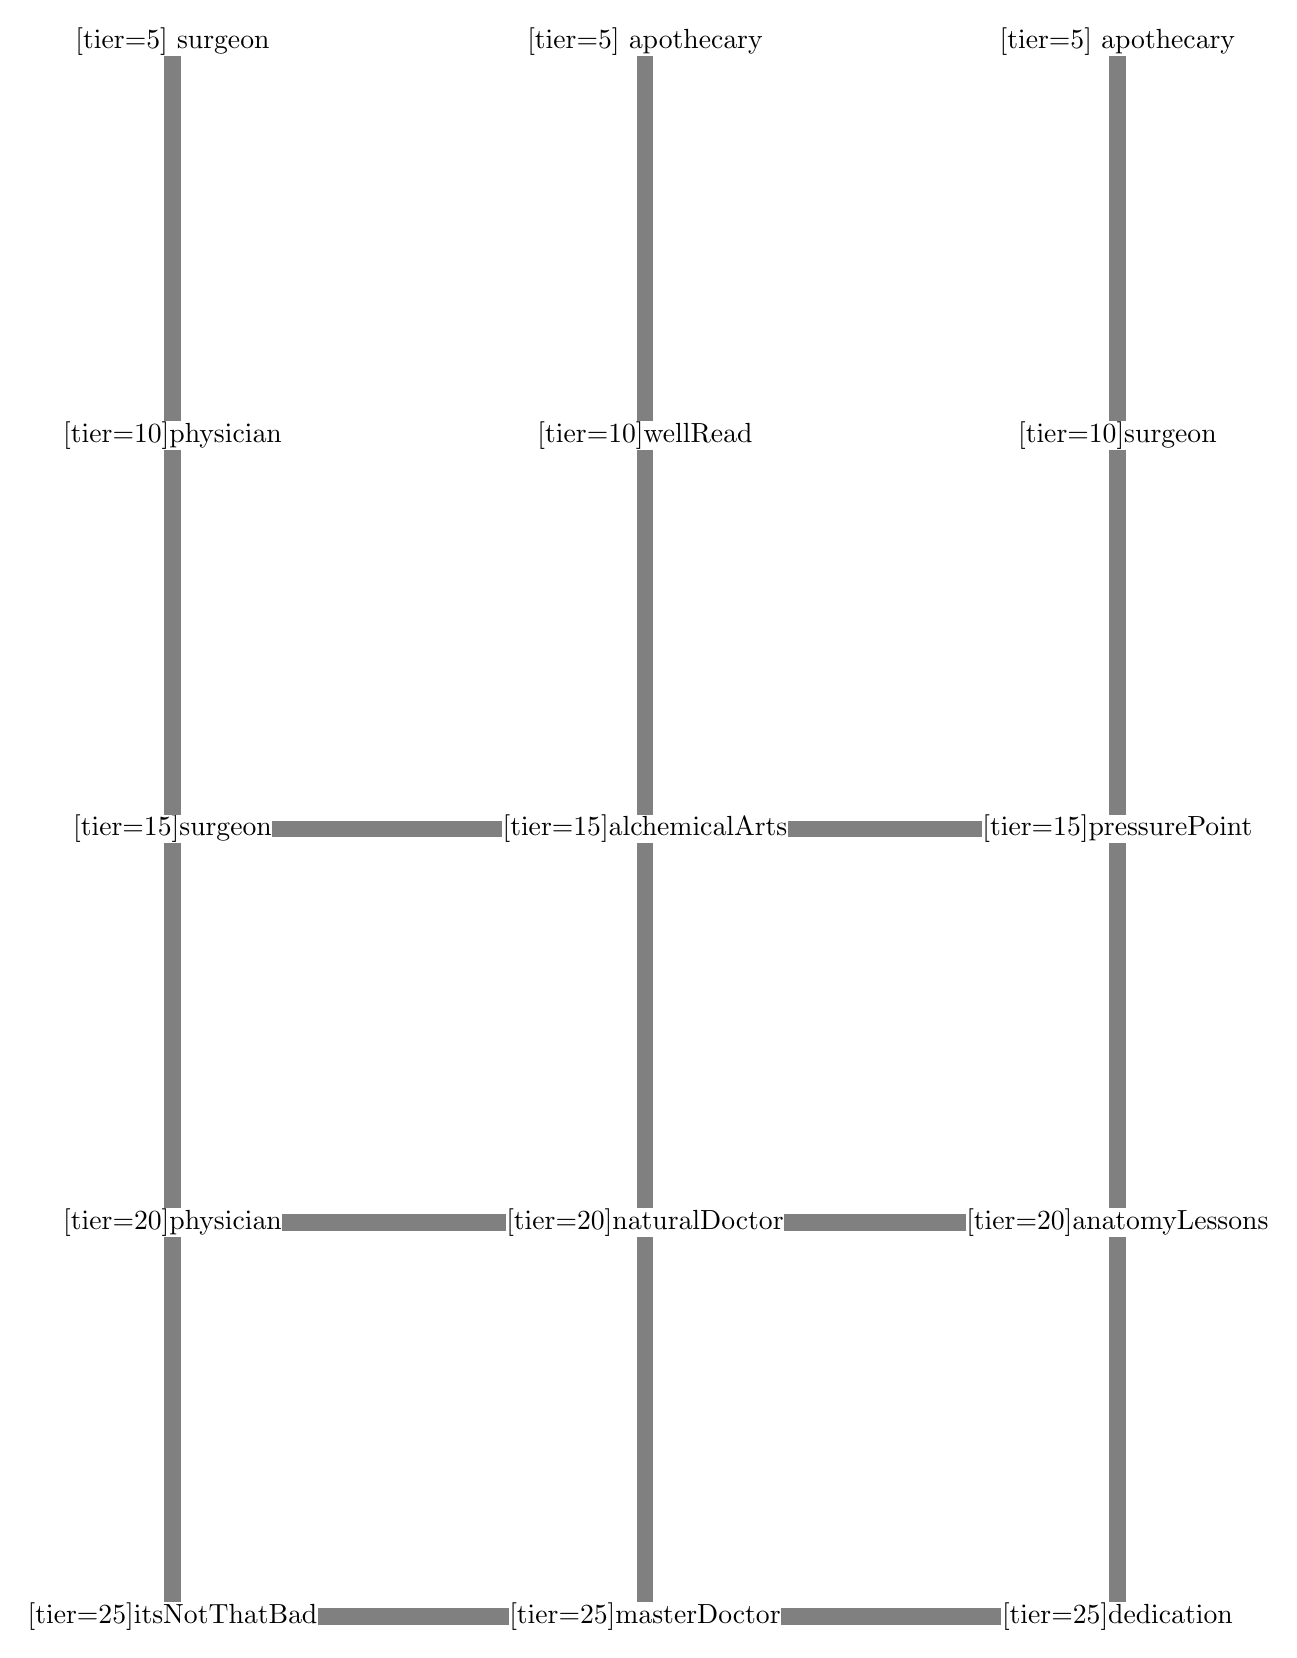
\begin{tikzpicture}
        \draw ( 0,  0) node(aa)[inner sep=0]{\TalentBox[tier=5] {surgeon}}
              ( 6,  0) node(ab)[inner sep=0]{\TalentBox[tier=5] {apothecary}}
              (12,  0) node(ac)[inner sep=0]{\TalentBox[tier=5] {apothecary}}
              ( 0, -5) node(ba)[inner sep=0]{\TalentBox[tier=10]{physician}}
              ( 6, -5) node(bb)[inner sep=0]{\TalentBox[tier=10]{wellRead}}
              (12, -5) node(bc)[inner sep=0]{\TalentBox[tier=10]{surgeon}}
              ( 0,-10) node(ca)[inner sep=0]{\TalentBox[tier=15]{surgeon}}
              ( 6,-10) node(cb)[inner sep=0]{\TalentBox[tier=15]{alchemicalArts}}
              (12,-10) node(cc)[inner sep=0]{\TalentBox[tier=15]{pressurePoint}}
              ( 0,-15) node(da)[inner sep=0]{\TalentBox[tier=20]{physician}}
              ( 6,-15) node(db)[inner sep=0]{\TalentBox[tier=20]{naturalDoctor}}
              (12,-15) node(dc)[inner sep=0]{\TalentBox[tier=20]{anatomyLessons}}
              ( 0,-20) node(ea)[inner sep=0]{\TalentBox[tier=25]{itsNotThatBad}}
              ( 6,-20) node(eb)[inner sep=0]{\TalentBox[tier=25]{masterDoctor}}
              (12,-20) node(ec)[inner sep=0]{\TalentBox[tier=25]{dedication}}
        ;

        \tikzstyle{bar}=[gray,-,>=stealth, line width=6pt]

        \draw [bar] (aa) to (ba);
        \draw [bar] (ab) to (bb);
        \draw [bar] (ac) to (bc);

        \draw [bar] (ba) to (ca);
        \draw [bar] (bb) to (cb);
        \draw [bar] (bc) to (cc);

        \draw [bar] (ca) to (da);
        \draw [bar] (cb) to (db);
        \draw [bar] (cc) to (dc);

        \draw [bar] (da) to (ea);
        \draw [bar] (db) to (eb);
        \draw [bar] (dc) to (ec);

        \draw [bar] (ca) to (cb);
        \draw [bar] (cc) to (cb);

        \draw [bar] (da) to (db);
        \draw [bar] (dc) to (db);

        \draw [bar] (ea) to (eb);
        \draw [bar] (ec) to (eb);
    \end{tikzpicture}
}
